%%%%%%%%%%%%%%%%%%%%%%%%%%%%%%%%%%%%%%%%%%%%%%%%%%%%%%%%%%%%
%%  This Beamer template was created by Cameron Bracken.
%%  Anyone can freely use or modify it for any purpose
%%  without attribution.
%%
%%  Last Modified: January 9, 2009
%%

\documentclass[xcolor=x11names,french]{beamer}

%% General document %%%%%%%%%%%%%%%%%%%%%%%%%%%%%%%%%%
\usepackage{graphicx}
\usepackage{tikz}
%%%%%%%%%%%%%%%%%%%%%%%%%%%%%%%%%%%%%%%%%%%%%%%%%%%%%%


%% Beamer Layout %%%%%%%%%%%%%%%%%%%%%%%%%%%%%%%%%%
\useoutertheme[subsection=false,shadow]{miniframes}
\useinnertheme{default}
\usefonttheme{professionalfonts}
\usepackage{palatino}
\usepackage{eurosym}
\usepackage{breqn}
\usepackage{hyperref}

\usepackage[french]{babel}
\selectlanguage{french}
\usepackage[T1]{fontenc}
\usepackage[utf8]{inputenc}
\usepackage{subcaption}

\setbeamerfont{title like}{shape=\scshape}
\setbeamerfont{frametitle}{shape=\scshape}
\setbeamertemplate{headline}{}


\setbeamercolor*{lower separation line head}{bg=DeepSkyBlue4} 
\setbeamercolor*{normal text}{fg=black,bg=white} 
\setbeamercolor*{alerted text}{fg=red} 
\setbeamercolor*{example text}{fg=black} 
\setbeamercolor*{structure}{fg=black} 
 
\setbeamercolor*{palette tertiary}{fg=black,bg=black!10} 
\setbeamercolor*{palette quaternary}{fg=black,bg=black!10} 

\renewcommand{\(}{\begin{columns}}
\renewcommand{\)}{\end{columns}}
\newcommand{\<}[1]{\begin{column}{#1}}
\renewcommand{\>}{\end{column}}


\usepackage{xcolor}	 % Required for custom colors
% Define a few colors for making text stand out within the presentation
\definecolor{mygreen}{RGB}{44,85,17}
\definecolor{myblue}{RGB}{0,51,102}
\definecolor{mybrown}{RGB}{194,164,113}
\definecolor{myred}{RGB}{255,66,56}


\usepackage{scrpage2} % Required for customization of the header and footer
\pagestyle{scrheadings} % Activates the pagestyle from scrpage2 for custom headers and footers
\clearscrheadfoot % Remove the default header and footer
%\setkomafont{pageheadfoot}{\normalfont\color{black}\sffamily} % Font settings for the header and footer


\newcommand\Wider[2][3em]{%
\makebox[\linewidth][c]{%
  \begin{minipage}{\dimexpr\textwidth+#1\relax}
  \raggedright#2
  \end{minipage}%
  }%
}


%\ifoot{% Left side
%\hspace{-2mm}
%\begin{tikzpicture}[remember picture,overlay]
%\node [xshift=\paperwidth/2, yshift=8.6cm] at (current page.south west)[
%rectangle, 
%fill, 
%inner sep=0pt, 
%minimum width=\paperwidth, 
%minimum height=1.5pt, top color=myblue, 
%bottom color=myblue
%]{}; % Green bar
%\end{tikzpicture}
%}

\setbeamertemplate{footline}[0]{}
%
%\usepackage{enumitem}
%\setlist[description]{leftmargin=1cm,labelindent=0.5cm}
%%%%%%%%%%%%%%%%%%%%%%%%%%%%%%%%%%%%%%%%%%%%%%%%%%




\begin{document}


%%%%%%%%%%%%%%%%%%%%%%%%%%%%%%%%%%%%%%%%%%%%%%%%%%%%%%
%%%%%%%%%%%%%%%%%%%%%%%%%%%%%%%%%%%%%%%%%%%%%%%%%%%%%%
\begin{frame}[plain]
\title{Stage M2 : les liens entre les inégalités et la croissance}
\author{
	Clément Henin
}
\titlepage

\begin{figure}

\includegraphics[scale=0.1]{logoixxi.pdf}
\end{figure}

\end{frame}


%%%%%%%%%%%%%%%%%%%%%%%%%%%%%%%%%%%%%%%%%%%%%%%%%%%%%%
%%%%%%%%%%%%%%%%%%%%%%%%%%%%%%%%%%%%%%%%%%%%%%%%%%%%%%
\begin{frame}{Publication OCDE}

\begin{figure}

\includegraphics[scale=0.2]{cover_OECD}
\end{figure}


\end{frame}


%%%%%%%%%%%%%%%%%%%%%%%%%%%%%%%%%%%%%%%%%%%%%%%%%%%%%%
%%%%%%%%%%%%%%%%%%%%%%%%%%%%%%%%%%%%%%%%%%%%%%%%%%%%%%
\begin{frame}{\'Equation empirique}

\begin{dmath}
ln y_{c, t} - ln y_{c, t - 1} = \alpha ln y_{c, t - 1} + \beta_1 Etudes_{c, t - 1} + \beta_2 Invest_{c, t - 1} + \gamma Gini_{c, t - 1} + \mu_{c} + \mu_{t} + \epsilon_{c, t}
\end{dmath}

Les coefficients sont estimés avec une méthode des moments généralisés \og système \fg{}. \\
Le jeu de données utilisé contient moins de 130 observations.

\end{frame}


%%%%%%%%%%%%%%%%%%%%%%%%%%%%%%%%%%%%%%%%%%%%%%%%%%%%%%
%%%%%%%%%%%%%%%%%%%%%%%%%%%%%%%%%%%%%%%%%%%%%%%%%%%%%%
\begin{frame}{Résultats}

\begin{figure}
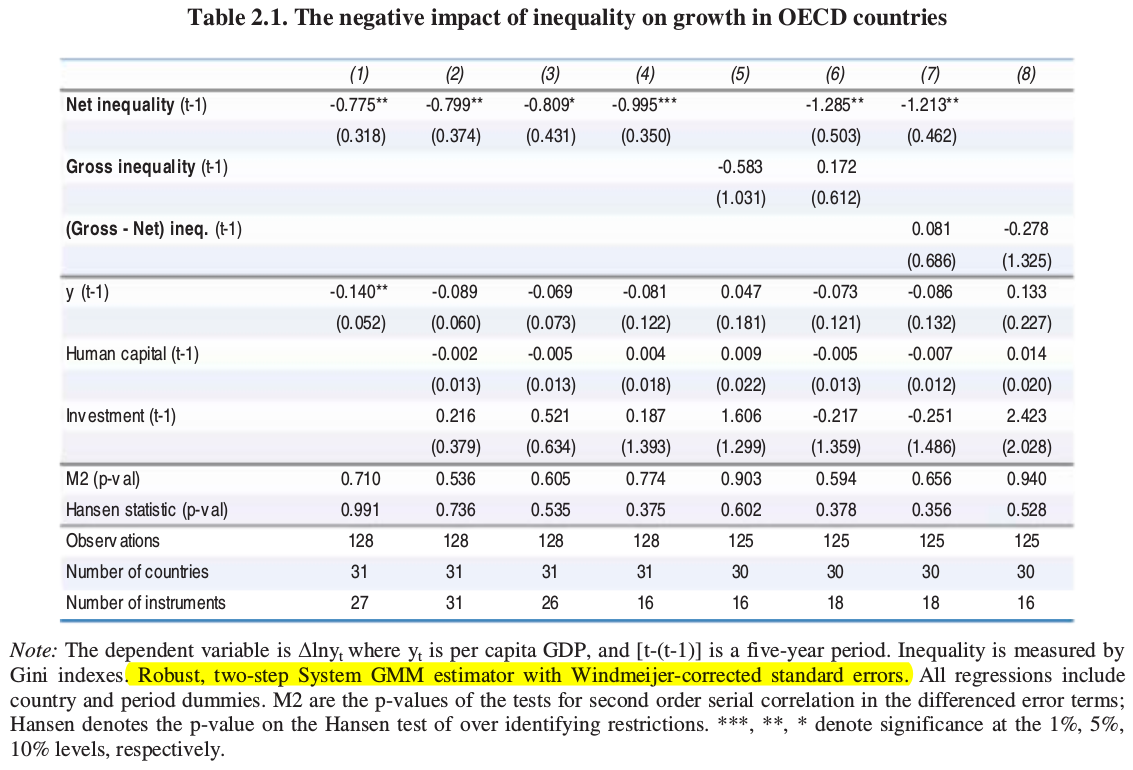
\includegraphics[scale=0.25]{OECD_regression_results}
\end{figure}

\end{frame}


%%%%%%%%%%%%%%%%%%%%%%%%%%%%%%%%%%%%%%%%%%%%%%%%%%%%%%
%%%%%%%%%%%%%%%%%%%%%%%%%%%%%%%%%%%%%%%%%%%%%%%%%%%%%%
\begin{frame}{Critique de Forbes (2000)}


Il n'y a pas assez de points pour se permettre un dummy par pays et par période. 


\begin{figure}
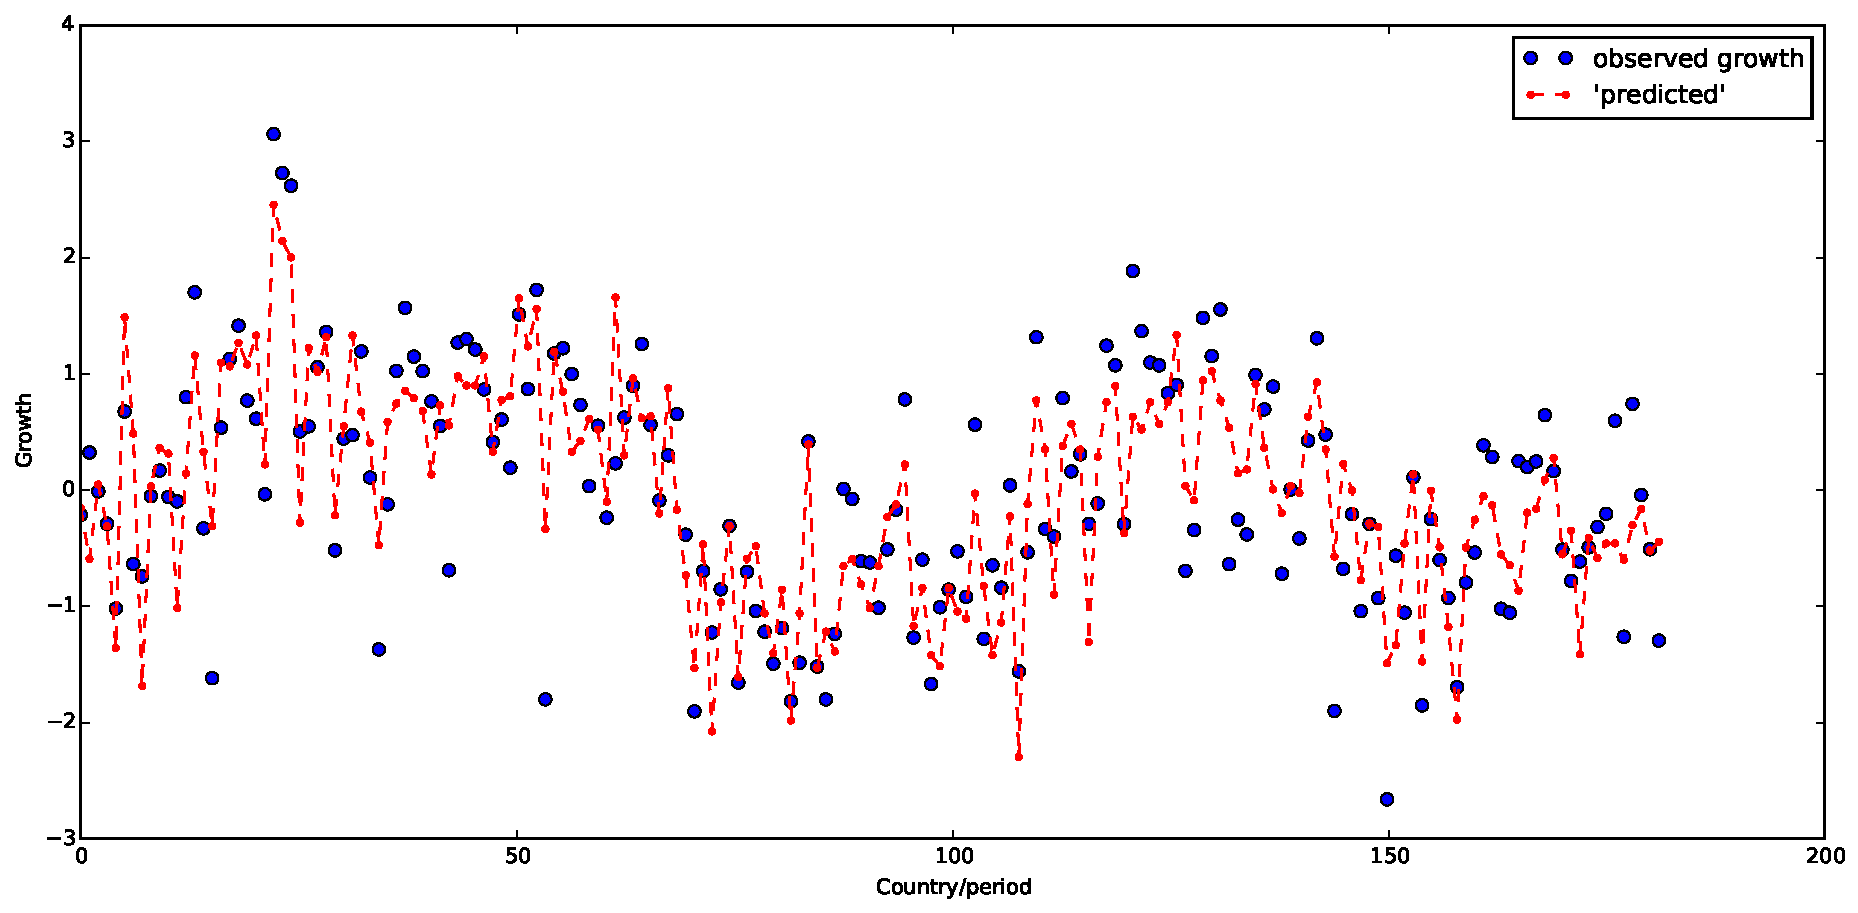
\includegraphics[scale=0.35]{OLS_results}
\caption{OLS avec des dummies}
\end{figure}

\end{frame}


%%%%%%%%%%%%%%%%%%%%%%%%%%%%%%%%%%%%%%%%%%%%%%%%%%%%%%
%%%%%%%%%%%%%%%%%%%%%%%%%%%%%%%%%%%%%%%%%%%%%%%%%%%%%%
\begin{frame}{Critique de Forbes (2000)}


Si on fait cette même régression en deux étapes on réalise quelle part de la variance est expliquée. 

\begin{figure}
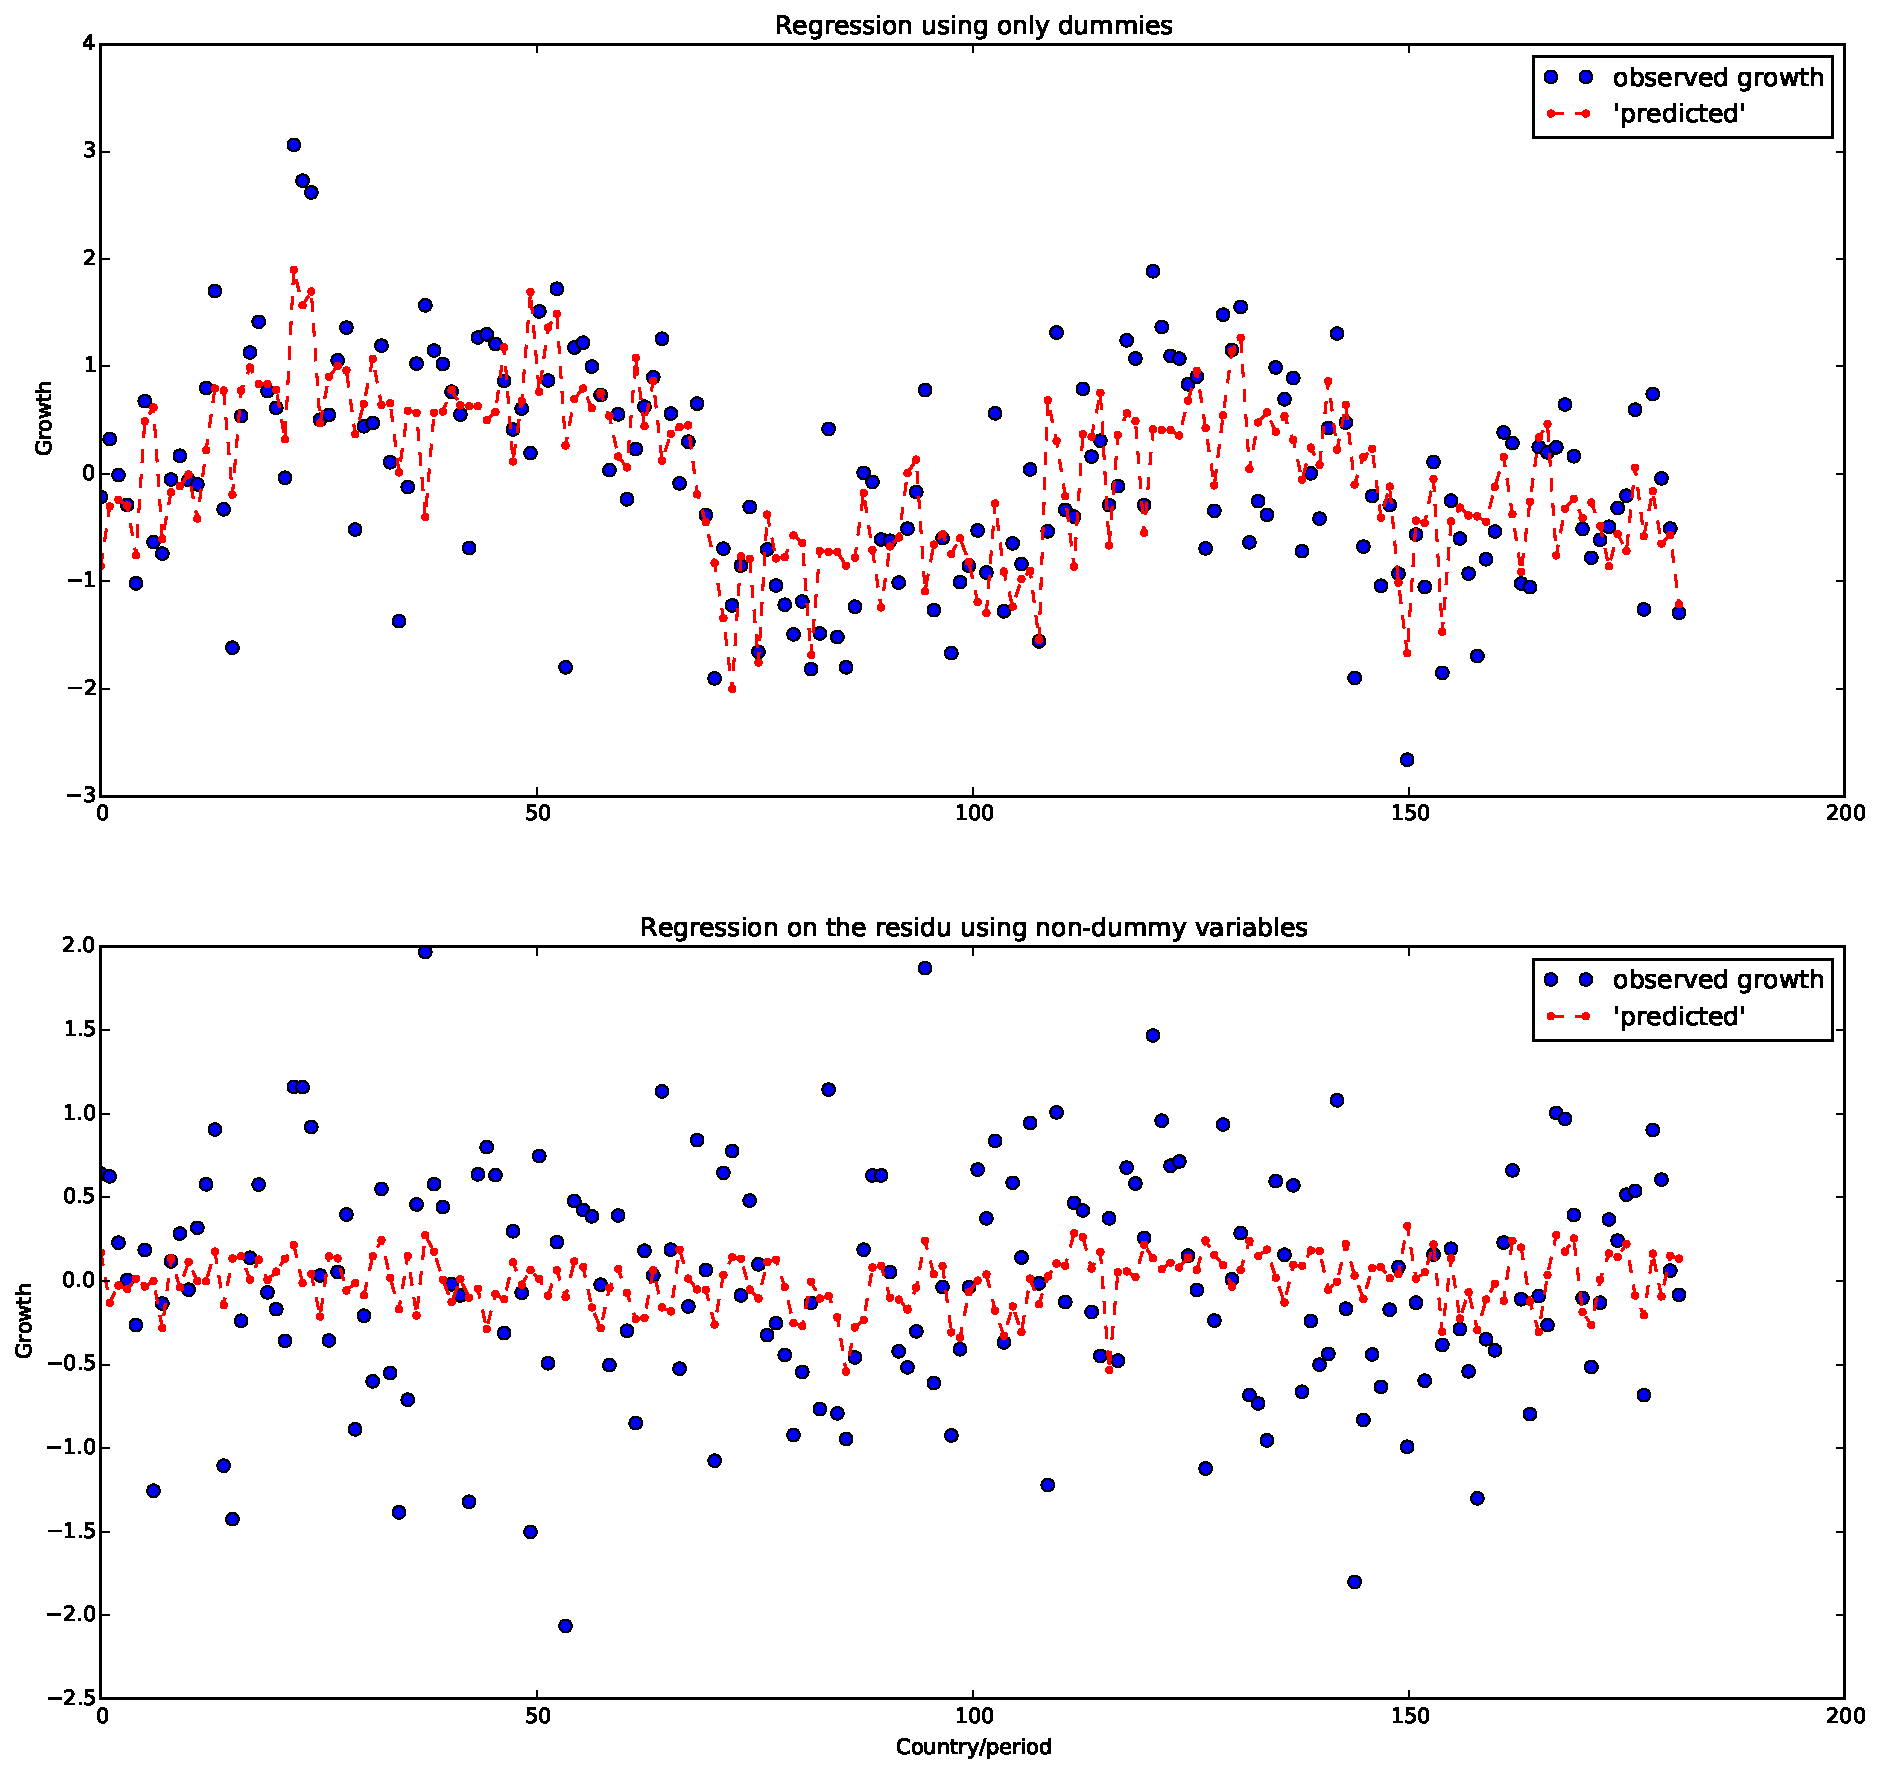
\includegraphics[scale=0.25]{two_steps_OLS}
\caption{OLS en deux étapes (1) seulement dummies (2) les autres variables}
\end{figure}

\end{frame}


%%%%%%%%%%%%%%%%%%%%%%%%%%%%%%%%%%%%%%%%%%%%%%%%%%%%%%
%%%%%%%%%%%%%%%%%%%%%%%%%%%%%%%%%%%%%%%%%%%%%%%%%%%%%%
\begin{frame}{Complexification}

On commence par discrétiser les variables : 

\begin{figure}
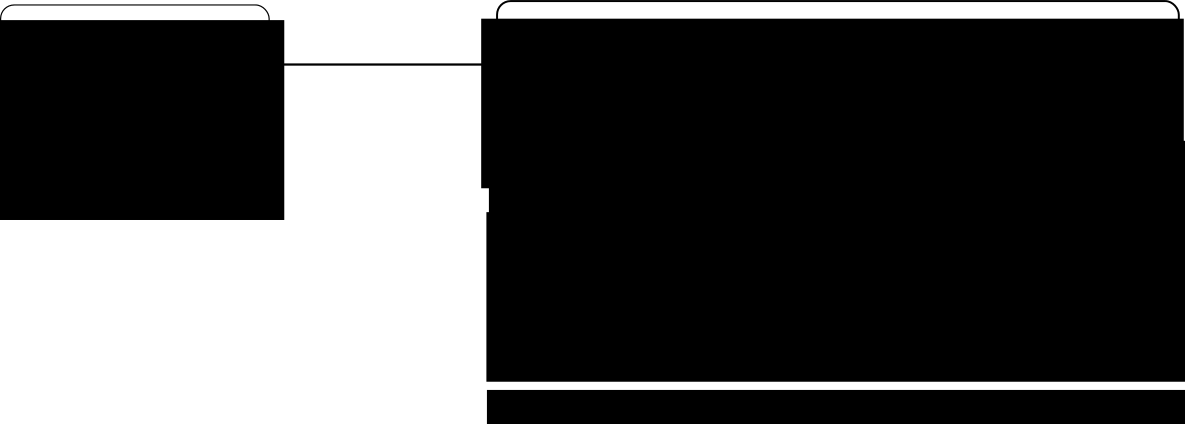
\includegraphics[scale=0.3]{quartilize}
\end{figure}


\end{frame}


%%%%%%%%%%%%%%%%%%%%%%%%%%%%%%%%%%%%%%%%%%%%%%%%%%%%%%
%%%%%%%%%%%%%%%%%%%%%%%%%%%%%%%%%%%%%%%%%%%%%%%%%%%%%%
\begin{frame}{QCA maison}

Impact des inégalités sur la croissance non pas en moyenne pour tous les pays mais plus spécifiquement.   \\
La croissance vaut 1 lorsque le pays.periode est dans le quart le plus fort. 
\bigskip

\begin{tabular}{c | c | c  c  c  }
     &        &       0     &      1    &   all \\
gini & gdp    &            &           &           \\
  \hline			
0  &  mean &  0.47222*** & 0.11956*** &  0.21875 \\
    & size  &        36   &       92   &    128 \\
1  &  mean & 0.39130***  &  0.14285* &  0.31343 \\
   &  size     &     92      &    42     &  134 \\
all & mean & 0.41406*** & 0.12686*** & 0.267176  \\
   &  size     &    128   &      134     &  262 \\
\end{tabular}

\bigskip

L'impact positif global du Gini vient simplement de la distribution gini-gdp ! 


\end{frame}


%%%%%%%%%%%%%%%%%%%%%%%%%%%%%%%%%%%%%%%%%%%%%%%%%%%%%%
%%%%%%%%%%%%%%%%%%%%%%%%%%%%%%%%%%%%%%%%%%%%%%%%%%%%%%
\begin{frame}{QCA maison}



\begin{tabular}{c | c | c  c  c  c }
    &        &    0      &  1      &     2     &  all \\
gini&  gdp    &            &          &            &    \\  
\hline
0  &   mean & 0.63636***  &  0.175 & 0.10606*** &  0.21875\\
    & size    &  22   &    40      &   66    &   128\\
1   & mean & 0.42424*** & 0.27906    &  0.08**  & 0.31343\\
    &  size     &     66   &    43     &     25    &   134\\
all & mean & 0.47727*** & 0.22891 & 0.09890*** & 0.267176\\
    & size    &      88  &     83     &     91    &   262 \\
\end{tabular}

\end{frame}


%%%%%%%%%%%%%%%%%%%%%%%%%%%%%%%%%%%%%%%%%%%%%%%%%%%%%%
%%%%%%%%%%%%%%%%%%%%%%%%%%%%%%%%%%%%%%%%%%%%%%%%%%%%%%
\begin{frame}{Arbre de décision}

Dans la lignée de la QCA, on a cherché une méthode permettant de trouver automatique des \og poches prévisibles \fg{} \textit{i.e.} des groupes pays.periode partageant les même caractéristiques et ayant une croissance moyenne significativement éloignée la moyenne globale. \\

\`A chaque étape, l'algorithme de régression trouve une division de l'espace des phases (variable, valeur) qui maxime \og l'homogénéité de chacun des groupes créés \fg{}. 

\[
R_1(j, s) = \{X / X_j < s\} \text{  and  } R_2(j, s) = \{X / X_j \ge s\}
\]

Avec $(j, s)$ solution de : 

\[
\min_{j, s}\Big[\min_{c_1} \sum_{x_i \in R_1(j,s)} (y_i - c_1)^2 + \min_{c_2} \sum_{x_i \in R_2(j,s)} (y_i - c_2)^2 \Big]
\]

\end{frame}


%%%%%%%%%%%%%%%%%%%%%%%%%%%%%%%%%%%%%%%%%%%%%%%%%%%%%%
%%%%%%%%%%%%%%%%%%%%%%%%%%%%%%%%%%%%%%%%%%%%%%%%%%%%%%
\begin{frame}{Exemple d'arbre}

\href{./exemple_arbre.pdf}{Arbre}

\end{frame}


%%%%%%%%%%%%%%%%%%%%%%%%%%%%%%%%%%%%%%%%%%%%%%%%%%%%%%
%%%%%%%%%%%%%%%%%%%%%%%%%%%%%%%%%%%%%%%%%%%%%%%%%%%%%%
\begin{frame}{Visualisation pour un arbre à 2 variables}

\begin{figure}
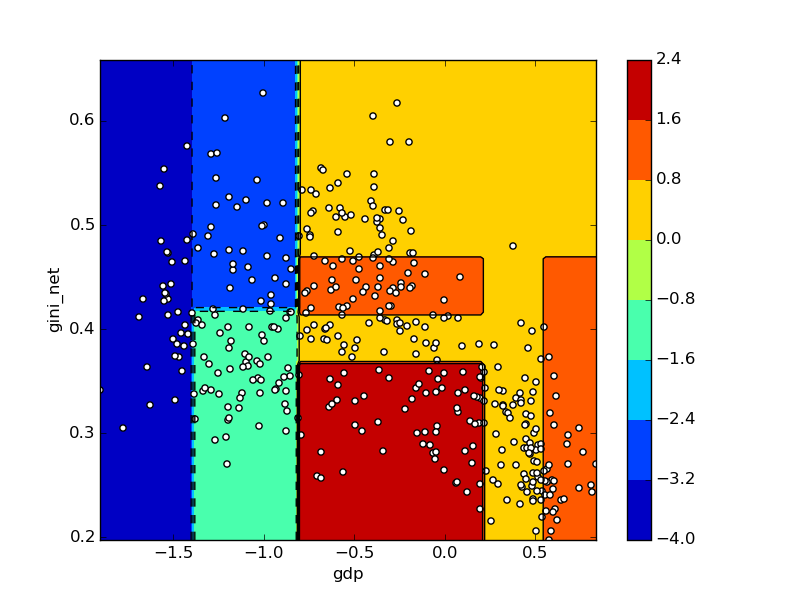
\includegraphics[scale=0.52]{decision_tree_vizualisation}
\end{figure}

\end{frame}


%%%%%%%%%%%%%%%%%%%%%%%%%%%%%%%%%%%%%%%%%%%%%%%%%%%%%%
%%%%%%%%%%%%%%%%%%%%%%%%%%%%%%%%%%%%%%%%%%%%%%%%%%%%%%
\begin{frame}{Encore à faire}

\begin{itemize}
\item Découper l'espace des phases en sous-groupe de pays partageant les mêmes caractéristiques et trouver l'influence du gini sur la croissance dans chacun de ces sous-groupes. \\
\bigskip
\href{./exemple_sous_groupe_pvalue.pdf}{Premier exemple} \\
\bigskip
\href{./gini-growth_correlations.pdf}{Qui donne}
\item Rechercher des différences entre groupes avec un découpage plus systématique (QCA maison avec différence de croissance en fonction du Gini à la place de la croissance)
\item améliorer la méthode pour la rendre plus robuste 
\end{itemize}


\end{frame}


%%%%%%%%%%%%%%%%%%%%%%%%%%%%%%%%%%%%%%%%%%%%%%%%%%%%%%
%%%%%%%%%%%%%%%%%%%%%%%%%%%%%%%%%%%%%%%%%%%%%%%%%%%%%%
\begin{frame}{Questions}

\begin{itemize}
\item corrélation croissance-PIB positive pour les deux variables à t et négative pour croissance à t et PIB à t - 1. Est-ce que cela ne vient pas simplement de la définition de la croissance ($PIB_t - PIB_{t - 1}$) ? Si oui, est-ce un problème ? Que faire alors ? (l'OCDE prend comme croissance la première croissance de la période de  années pour éviter cette corrélation)
\item Sur quelles autres variables pourrait-on utiliser notre méthode de QCA maison ? 
\end{itemize}

\end{frame}

\end{document}